\newcounter{UC}
\newcounter{SUC}
\newcounter{SSUC}

\newcommand{\resetCounter}[1]{%
    \setcounter{#1}{0}
}

\newcommand{\UseCase}[1]{%
    \refstepcounter{UC}
    \resetCounter{SUC}
    \resetCounter{SSUC}
    \subsection{UC\arabic{UC} - #1}\label{UC:\arabic{UC}}
}

\newcommand{\SubUseCase}[1]{%
    \stepcounter{SUC}
    \subsubsection{UC\arabic{UC}.\arabic{SUC} - #1}
}

\newcommand{\SubSubUseCase}[1]{%
    \stepcounter{SSUC}  
    \paragraph{UC\arabic{UC}.\arabic{SUC}.\arabic{SSUC} - #1}
}

% COME UTILIZZARE I CASI D`USO:
% i comandi di use case vanno utilizzati al posto di subsection, subsubsection e paragraph

% \UseCase => rappresenta lo use case principale (UC1,UC2,UC3)
% \SubUseCase => rappresenta il primo sotto livello dello use case principale (UC1.1,UC2.1,UC3.3)
% \SubSubUseCase => rappresenta il secondo sotto livello dello lo use case principale (UC1.1.1,UC2.1.2,UC3.3.1)

\newcommand{\UCdsc}[5]{
    \begin{itemize}
        \item \textbf{Attore primario:}
         #1
        \item \textbf{Descrizione:} 
         #2
        \item \textbf{Precondizioni:}
         #3
        \item \textbf{Postcondizioni:}
        #4
        \item \textbf{Scenario principale:} 
         #5
    \end{itemize}
}


\GetTitleStringSetup{expand}
\section{Casi d'uso}
% \subsection{Attore}
% Poiché per lo svolgimento del progetto non è necessario gestire permessi differenti per l'accesso alle funzionalità, l'attore che interagisce con il nostro software è unico, denominato "Utente".\\
% \textbf{Utente:} soggetto che utilizza la web application, sfruttandone le funzionalità.

\UseCase{Visualizza lista dataset}
    \begin{figure}[h!]
        \centering
        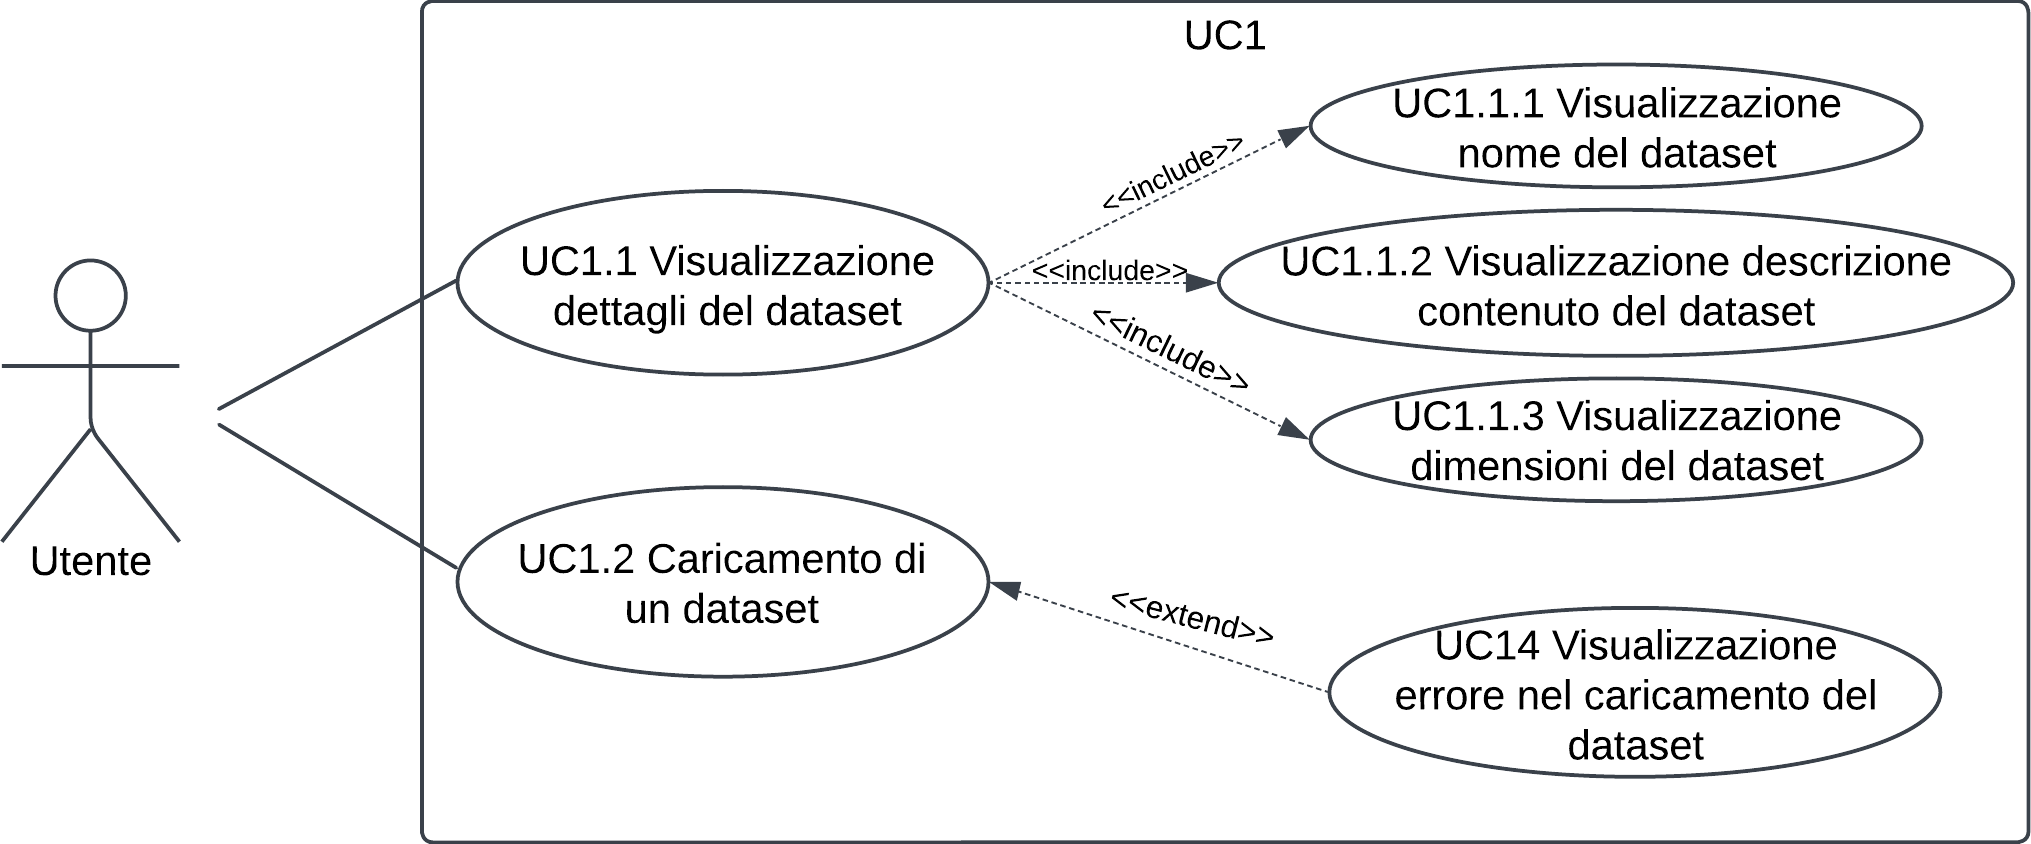
\includegraphics[scale=0.55]{template/images/UC1.png}
        \caption{\nameref*{UC:\arabic{UC}}}
    \end{figure}
    \UCdsc
    { % ATTORE
        \begin{itemize}
            \item Utente in homepage.
        \end{itemize}
    }
    { % DESCRIZIONE
        \begin{itemize}
            \item All'avvio del sistema l'utente visualizza la completa lista dei dataset proposti.
        \end{itemize}
    }
    { % PRECONDIZIONI
        \begin{itemize}
            \item L'utente ha accesso all'applicazione.
        \end{itemize}
    }
    { % POSTCONDIZIONI
        \begin{itemize}
            \item L'utente vede la lista dei dataset disponibili.
        \end{itemize}
    }
    { % SCENARIO PRIMARIO
        \begin{itemize}
            \item L'utente avvia il sistema;
            \item I dataset disponibili vengono presentati tramite un elenco;
        \end{itemize}
    }


    \newpage

    \SubUseCase{Visualizza singolo dataset}
    \UCdsc
    { % ATTORE
        \begin{itemize}
            \item Utente in homepage.
        \end{itemize}
    }
    { % DESCRIZIONE
        \begin{itemize}
            \item Visualizzazione dei singoli dataset di cui la lista è composta.
        \end{itemize}
    }
    { % PRECONDIZIONI
        \begin{itemize}
            \item La lista dei dataset è visibile.
        \end{itemize}
    }
    { % POSTCONDIZIONI
        \begin{itemize}
            \item La lista dei dataset è visibile;
            \item Il dataset è visibile nella lista dei dataset.
        \end{itemize}
    }
    { % SCENARIO PRIMARIO
        \begin{itemize}
            \item Nessuna azione richiesta;
        \end{itemize}
    }

    \SubSubUseCase{Visualizza nome dataset}
    \UCdsc
    { % ATTORE
        \begin{itemize}
            \item Utente in homepage.
        \end{itemize}
    }
    { % DESCRIZIONE
        \begin{itemize}
            \item Visualizzazione del nome del dataset. Quest'ultimo è considerato come un identificativo che permette di distinguere i diversi dataset.
        \end{itemize}
    }
    { % PRECONDIZIONI
        \begin{itemize}
            \item Il dataset è presente della lista dei dataset.
        \end{itemize}
    }
    { % POSTCONDIZIONI
        \begin{itemize}
            \item Il dataset è presente della lista dei dataset;
            \item Il nome del dataset è visibile.
        \end{itemize}
    }
    { % SCENARIO PRIMARIO
        \begin{itemize}
            \item Nessuna azione richiesta;
        \end{itemize}
    }


    \SubSubUseCase{Visualizza dimensione dataset}
    \UCdsc
    { % ATTORE
        \begin{itemize}
            \item Utente in homepage.
        \end{itemize}
    }
    { % DESCRIZIONE
        \begin{itemize}
            \item Visualizzazione della dimensione del dataset.
        \end{itemize}
    }
    { % PRECONDIZIONI
        \begin{itemize}
            \item Il dataset è presente della lista dei dataset.
        \end{itemize}
    }
    { % POSTCONDIZIONI
        \begin{itemize}
            \item Il dataset è presente della lista dei dataset;
            \item La dimensione del dataset è visibile.
        \end{itemize}
    }
    { % SCENARIO PRIMARIO
        \begin{itemize}
            \item Nessuna azione richiesta;
        \end{itemize}
    }


\UseCase{Visualizza dettaglio dataset}
    \begin{figure}[h!]
        \centering
        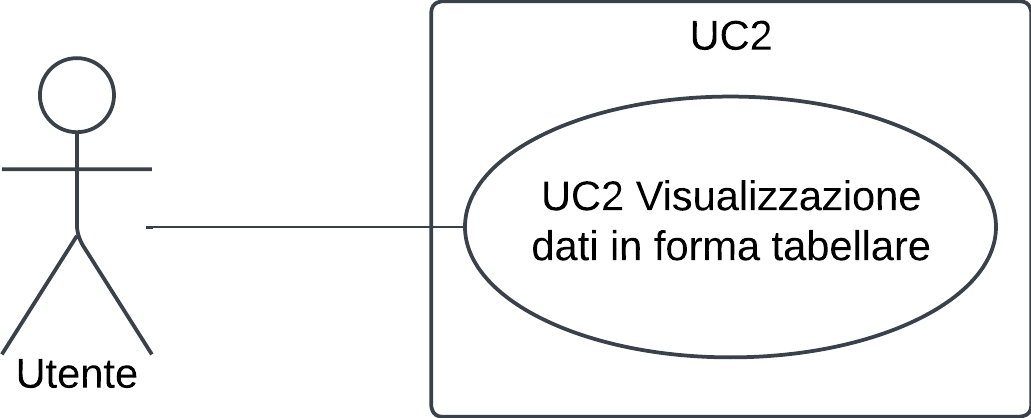
\includegraphics[scale=0.6]{template/images/UC2.png}
        \caption{\nameref*{UC:\arabic{UC}}}
    \end{figure}
    \UCdsc
    { % ATTORE
        \begin{itemize}
            \item Utente in homepage.
        \end{itemize}
    }
    { % DESCRIZIONE
        \begin{itemize}
            \item  L'utente può visualizzare i dettagli di un dataset.
        \end{itemize}
    }
    { % PRECONDIZIONI
        \begin{itemize}
            \item Il dataset deve essere un dataset proposto.
        \end{itemize}
    }
    { % POSTCONDIZIONI
        \begin{itemize}
            \item I dettagli del dataset sono visibili.
        \end{itemize}
    }
    { % SCENARIO PRIMARIO
        \begin{itemize}
            \item L'utente espande la vista del singolo dataset;
        \end{itemize}
    }
    

    \SubUseCase{Visualizza descrizione dataset}
    \UCdsc
    { % ATTORE
        \begin{itemize}
            \item Utente in homepage.
        \end{itemize}
    }
    { % DESCRIZIONE
        \begin{itemize}
            \item   Visualizzazione della descrizione del dataset.
        \end{itemize}
    }
    { % PRECONDIZIONI
        \begin{itemize}
            \item I dettagli del dataset sono visibili.
        \end{itemize}
    }
    { % POSTCONDIZIONI
        \begin{itemize}
            \item I dettagli del dataset sono visibili.
            \item La descrizione del dataset è visibile.
        \end{itemize}
    }
    { % SCENARIO PRIMARIO
        \begin{itemize}
            \item Nessuna azione richiesta;
        \end{itemize}
    }



\UseCase{Carica dataset}
\begin{figure}[h!]
    \centering
    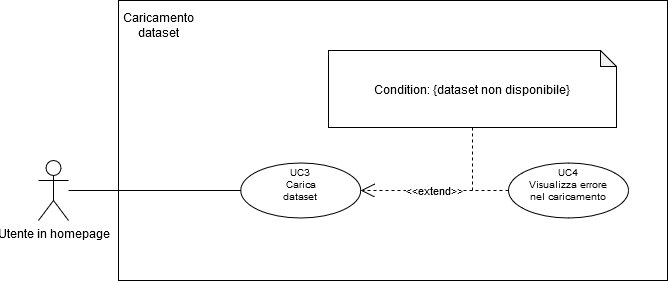
\includegraphics[scale=0.6]{template/images/UC3.png}
    \caption{\nameref*{UC:\arabic{UC}}}
\end{figure}
    \UCdsc
    { % ATTORE
        \begin{itemize}
            \item Utente in homepage.
        \end{itemize}
    }
    { % DESCRIZIONE
        \begin{itemize}
            \item  L'utente decide il dataset che vuole visualizzare andando quindi a caricare tutti i dati e valori nel sistema.
        \end{itemize}
    }
    { % PRECONDIZIONI
        \begin{itemize}
            \item L'utente vede la lista dei dataset disponibili.
            \item L'utente ha selezionato un dataset.
        \end{itemize}
    }
    { % POSTCONDIZIONI
        \begin{itemize}
            \item L'utente ha selezionato un dataset.
            \item Il dataset viene caricato nel sistema.
            \item L'utente entra nell'ambiente 3D
        \end{itemize}
    }
    { % SCENARIO PRIMARIO
        \begin{itemize}
            \item L'utente seleziona un dataset tra quelli proposti nella lista;
        \end{itemize}
        % ESTENSIONE
        \item \textbf{Estensione:} \begin{itemize}
            \item UC4 - Visualizza errore nel caricamento.
        \end{itemize}
    }


\newpage

\UseCase{Visualizza errore nel caricamento}
    \UCdsc
    { % ATTORE
        \begin{itemize}
            \item Utente in homepage.
        \end{itemize}
    }
    { % DESCRIZIONE
        \begin{itemize}
            \item  Visualizzazione di un messaggio informativo "oggetto non modificabile". Il caricamento potrebbe fallire perchè il dataset selezionato potrebbe essere
                    non disponibile in quel momento.
        \end{itemize}
    }
    { % PRECONDIZIONI
        \begin{itemize}
            \item L'utente vede la lista dei dataset disponibili;
            \item L'utente ha selezionato un dataset;
            \item Il dataset selezionato non è disponibile.
        \end{itemize}
    }
    { % POSTCONDIZIONI
        \begin{itemize}
            \item Il dataset non viene caricato nel sistema.
            \item L'utente torna alla vista della lista di dataset.
        \end{itemize}
    }
    { % SCENARIO PRIMARIO
        \begin{itemize}
            \item L'utente seleziona un dataset tra quelli proposti nella lista;
        \end{itemize}
    }



\UseCase{Visualizza dataset in forma tabellare}
\begin{figure}[h!]
    \centering
    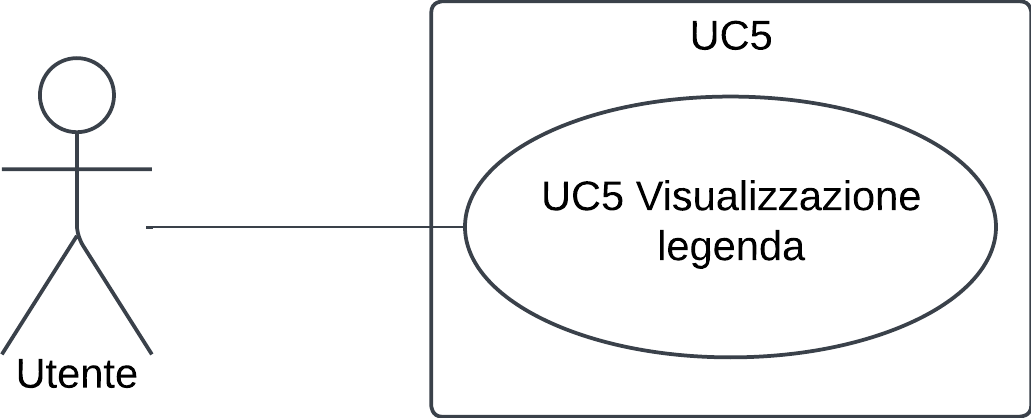
\includegraphics[scale=0.7]{template/images/UC5.png}
    \caption{\nameref*{UC:\arabic{UC}}}
\end{figure}
\UCdsc
    { % ATTORE
        \begin{itemize}
            \item Utente in ambiente 3D.
        \end{itemize}
    }
    { % DESCRIZIONE
        \begin{itemize}
            \item Visualizzazione del dataset caricato in forma tabellare.
        \end{itemize}
    }
    { % PRECONDIZIONI
        \begin{itemize}
            \item L'utente ha selezionato un dataset;
            \item Il caricamento del dataset è andato a buonfine;
            \item L'utente è all'interno dell'ambiente 3D.
        \end{itemize}
    }
    { % POSTCONDIZIONI
        \begin{itemize}
            \item La tabella contenente i dati del dataset è visibile con i rispettivi valori.
        \end{itemize}
    }
    { % SCENARIO PRIMARIO
        \begin{itemize}
            \item L'utente seleziona un dataset;
            \item L'applicazione elabora i dati.
        \end{itemize}
    }


\SubUseCase{Visualizza intestazioni}
\UCdsc
    { % ATTORE
        \begin{itemize}
            \item Utente in ambiente 3D.
        \end{itemize}
    }
    { % DESCRIZIONE
        \begin{itemize}
            \item Visualizzazione delle intestazioni della tabella contenente i tutti i valori del dataset selezionato.
        \end{itemize}
    }
    { % PRECONDIZIONI
        \begin{itemize}
            \item La tabella è visibile;
        \end{itemize}
    }
    { % POSTCONDIZIONI
        \begin{itemize}
            \item Le intestazioni della tabella sono visibili.
        \end{itemize}
    }
    { % SCENARIO PRIMARIO
        \begin{itemize}
            \item Nessuna azione richiesta;
        \end{itemize}
    }

\SubUseCase{Visualizza dati}
\UCdsc
    { % ATTORE
        \begin{itemize}
            \item Utente in ambiente 3D.
        \end{itemize}
    }
    { % DESCRIZIONE
        \begin{itemize}
            \item Visualizzazione di tutti i valori, del dataset selezionato, contenuti nella tabella.
        \end{itemize}
    }
    { % PRECONDIZIONI
        \begin{itemize}
            \item La tabella è visibile;
        \end{itemize}
    }
    { % POSTCONDIZIONI
        \begin{itemize}
            \item I valori del dataset selezionato vengono visualizzati nella tabella.
        \end{itemize}
    }
    { % SCENARIO PRIMARIO
        \begin{itemize}
            \item Nessuna azione richiesta;
        \end{itemize}
    }

\UseCase{Visualizza dataset tramite grafico 3D}
\begin{figure}[h!]
    \centering
    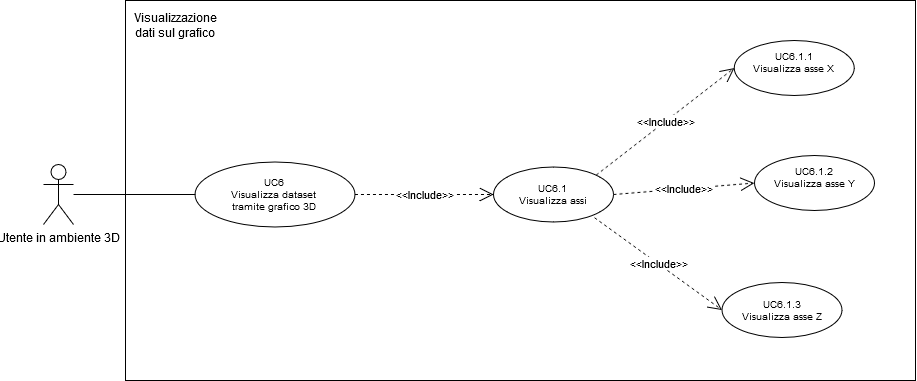
\includegraphics[scale=0.5]{template/images/UC6.png}
    \caption{\nameref*{UC:\arabic{UC}}}
\end{figure}
\UCdsc
    { % ATTORE
        \begin{itemize}
            \item Utente in ambiente 3D.
        \end{itemize}
    }
    { % DESCRIZIONE
        \begin{itemize}
            \item Visualizzazione del dataset caricato sotto forma di grafico 3D a barre verticale.
        \end{itemize}
    }
    { % PRECONDIZIONI
        \begin{itemize}
            \item L'utente ha selezionato un dataset;
            \item Il caricamento del dataset è andato a buonfine;
            \item L'utente è all'interno dell'ambiente 3D.
        \end{itemize}
    }
    { % POSTCONDIZIONI
        \begin{itemize}
            \item Il grafico 3D è visibile.
        \end{itemize}
    }
    { % SCENARIO PRIMARIO
        \begin{itemize}
            \item L'utente seleziona un dataset;
            \item L'applicazione elabora i dati.
        \end{itemize}
    }




\SubUseCase{Visualizza assi}
\UCdsc
    { % ATTORE
        \begin{itemize}
            \item Utente in ambiente 3D.
        \end{itemize}
    }
    { % DESCRIZIONE
        \begin{itemize}
            \item Visualizzazione degli asse X, Y e Z del grafico 3D.
        \end{itemize}
    }
    { % PRECONDIZIONI
        \begin{itemize}
            \item Il grafico 3D è visibile;
        \end{itemize}
    }
    { % POSTCONDIZIONI
        \begin{itemize}
            \item Gli assi del grafico 3D sono visibili.
        \end{itemize}
    }
    { % SCENARIO PRIMARIO
        \begin{itemize}
            \item Nessuna azione richiesta;
        \end{itemize}
    }

\SubSubUseCase{Visualizza asse X}
\UCdsc
    { % ATTORE
        \begin{itemize}
            \item Utente in ambiente 3D.
        \end{itemize}
    }
    { % DESCRIZIONE
        \begin{itemize}
            \item Visualizzazione degli asse X del grafico 3D con le sue eventuali etichette.
        \end{itemize}
    }
    { % PRECONDIZIONI
        \begin{itemize}
            \item Il grafico 3D è visibile;
        \end{itemize}
    }
    { % POSTCONDIZIONI
        \begin{itemize}
            \item L'asse X del grafico 3D è visibile.
        \end{itemize}
    }
    { % SCENARIO PRIMARIO
        \begin{itemize}
            \item Nessuna azione richiesta;
        \end{itemize}
    }

\SubSubUseCase{Visualizza asse X}
\UCdsc
    { % ATTORE
        \begin{itemize}
            \item Utente in ambiente 3D.
        \end{itemize}
    }
    { % DESCRIZIONE
        \begin{itemize}
            \item Visualizzazione degli asse Y del grafico 3D con le sue eventuali etichette.
        \end{itemize}
    }
    { % PRECONDIZIONI
        \begin{itemize}
            \item Il grafico 3D è visibile;
        \end{itemize}
    }
    { % POSTCONDIZIONI
        \begin{itemize}
            \item L'asse Y del grafico 3D è visibile.
        \end{itemize}
    }
    { % SCENARIO PRIMARIO
        \begin{itemize}
            \item Nessuna azione richiesta;
        \end{itemize}
    }

\SubSubUseCase{Visualizza asse Z}
\UCdsc
    { % ATTORE
        \begin{itemize}
            \item Utente in ambiente 3D.
        \end{itemize}
    }
    { % DESCRIZIONE
        \begin{itemize}
            \item Visualizzazione degli asse Z del grafico 3D con le sue eventuali etichette.
        \end{itemize}
    }
    { % PRECONDIZIONI
        \begin{itemize}
            \item Il grafico 3D è visibile;
        \end{itemize}
    }
    { % POSTCONDIZIONI
        \begin{itemize}
            \item L'asse Z del grafico 3D è visibile.
        \end{itemize}
    }
    { % SCENARIO PRIMARIO
        \begin{itemize}
            \item Nessuna azione richiesta;
        \end{itemize}
    }

\UseCase{Camera Panning}
\begin{figure}[h!]
    \centering
    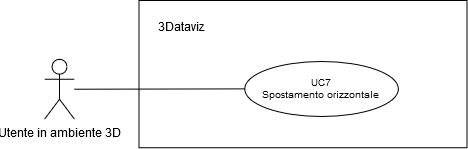
\includegraphics[scale=0.65]{template/images/UC7.png}
    \caption{\nameref*{UC:\arabic{UC}}}
\end{figure}
\UCdsc
    { % ATTORE
        \begin{itemize}
            \item Utente in ambiente 3D.
        \end{itemize}
    }
    { % DESCRIZIONE
        \begin{itemize}
            \item Compiere movimenti di pan significa che, l'utente può interagire con l'ambiente compiendo degli spostamenti lungo una linea retta mantenendo la stessa angolazione.
        \end{itemize}
    }
    { % PRECONDIZIONI
        \begin{itemize}
            \item Le azioni di movimento devono essere valide. Un'azione di movimento è valida se non va al di fuori di un'area predefinita dal sistema;
            \item La telecamera si trova in una posizione arbitraria nello spazio.
        \end{itemize}
    }
    { % POSTCONDIZIONI
        \begin{itemize}
            \item La telecamera si trova in una posizione diversa da quella iniziale.
        \end{itemize}
    }
    { % SCENARIO PRIMARIO
        \begin{itemize}
            \item L'utente interagisce con il sistema per compiere un'azione di movimento di spostamento orizzontale e/o verticale;
        \end{itemize}
    }

\SubUseCase{Spostamento orizzontale}
    \UCdsc
        { % ATTORE
            \begin{itemize}
                \item Utente in ambiente 3D.
            \end{itemize}
        }
        { % DESCRIZIONE
            \begin{itemize}
                \item Compiere movimenti di pan significa che, l'utente può interagire con l'ambiente compiendo degli spostamenti orizzontali indipendentemente dalla sua angolazione.
            \end{itemize}
        }
        { % PRECONDIZIONI
            \begin{itemize}
                \item Le azioni di movimento devono essere valide. Un'azione di movimento è valida se non va oltre il margine destro o sinistro di un'area predefinita dal sistema;
                \item La telecamera si trova in una posizione arbitraria nello spazio.
            \end{itemize}
        }
        { % POSTCONDIZIONI
            \begin{itemize}
                \item La telecamera si trova in una posizione diversa da quella iniziale.
            \end{itemize}
        }
        { % SCENARIO PRIMARIO
            \begin{itemize}
                \item L'utente interagisce con il sistema per compiere un'azione di movimento di spostamento orizzontale;
            \end{itemize}
        }

\SubUseCase{Spostamento orizzontale}
    \UCdsc
        { % ATTORE
            \begin{itemize}
                \item Utente in ambiente 3D.
            \end{itemize}
        }
        { % DESCRIZIONE
            \begin{itemize}
                \item Compiere movimenti di pan significa che, l'utente può interagire con l'ambiente compiendo degli spostamenti verticali indipendentemente dalla sua angolazione.
            \end{itemize}
        }
        { % PRECONDIZIONI
            \begin{itemize}
                \item Le azioni di movimento devono essere valide. Un'azione di movimento è valida se non va al di sotto o al di sopra di un'area predefinita dal sistema;
                \item La telecamera si trova in una posizione arbitraria nello spazio.
            \end{itemize}
        }
        { % POSTCONDIZIONI
            \begin{itemize}
                \item La telecamera si trova in una posizione diversa da quella iniziale.
            \end{itemize}
        }
        { % SCENARIO PRIMARIO
            \begin{itemize}
                \item L'utente interagisce con il sistema per compiere un'azione di movimento di spostamento verticale;
            \end{itemize}
        }


\UseCase{Zoom della vista}
\begin{figure}[h!]
    \centering
    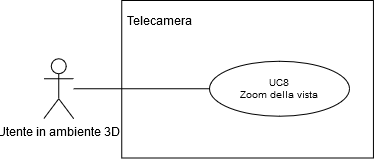
\includegraphics[scale=0.7]{template/images/UC8.png}
    \caption{\nameref*{UC:\arabic{UC}}}
\end{figure}
\UCdsc
{ % ATTORE
    \begin{itemize}
        \item Utente in ambiente 3D.
    \end{itemize}
}
{ % DESCRIZIONE
    \begin{itemize}
        \item Compiere movimenti di zoom significa che, l'utente può interagire con l'ambiente compiendo degli spostamenti in profondità.
    \end{itemize}
}
{ % PRECONDIZIONI
    \begin{itemize}
        \item L'azione di zoom deve essere valida. Un'azione di zoom è valida se non va al di fuori un'area predefinita dal sistema;
        \item La telecamera si trova in una posizione arbitraria nello spazio.
    \end{itemize}
}
{ % POSTCONDIZIONI
    \begin{itemize}
        \item La telecamera si trova in una posizione diversa da quella iniziale in termini di profondità.
    \end{itemize}
}
{ % SCENARIO PRIMARIO
    \begin{itemize}
        \item L'utente interagisce con il sistema per compiere un'azione zoom;
    \end{itemize}
}

\UseCase{Ruota grafico}
\begin{figure}[h!]
    \centering
    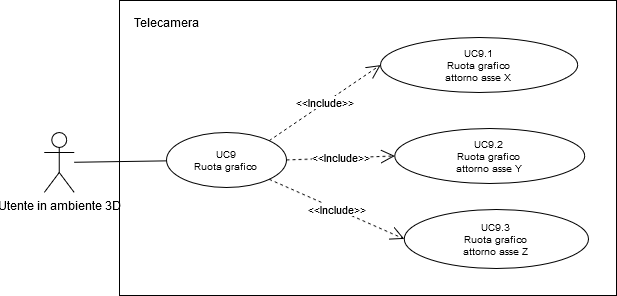
\includegraphics[scale=0.65]{template/images/UC9.png}
    \caption{\nameref*{UC:\arabic{UC}}}
\end{figure}
\UCdsc
{ % ATTORE
    \begin{itemize}
        \item Utente in ambiente 3D.
    \end{itemize}
}
{ % DESCRIZIONE
    \begin{itemize}
        \item Compiere un'azione di rotazione del grafico permette all'utente di visualizzare meglio o con una angolazione che preferisce il grafico stesso.
    \end{itemize}
}
{ % PRECONDIZIONI
    \begin{itemize}
        \item Il grafico è visibile;
        \item Il grafico ha una rotazione arbitraria.
    \end{itemize}
}
{ % POSTCONDIZIONI
    \begin{itemize}
        \item Il grafico ha una rotazione diversa rispetto a quella iniziale.
    \end{itemize}
}
{ % SCENARIO PRIMARIO
    \begin{itemize}
        \item L'utente interagisce con il sistema per compiere di rotazione del grafico.
    \end{itemize}
}

\SubUseCase{Ruota grafico attorno asse X}
\UCdsc
{ % ATTORE
    \begin{itemize}
        \item Utente in ambiente 3D.
    \end{itemize}
}
{ % DESCRIZIONE
    \begin{itemize}
        \item L'attore compie un'azione di rotazione del grafico attorno l'asse X.
    \end{itemize}
}
{ % PRECONDIZIONI
    \begin{itemize}
        \item Il grafico è visibile;
        \item Il grafico ha una rotazione arbitraria.
    \end{itemize}
}
{ % POSTCONDIZIONI
    \begin{itemize}
        \item Il grafico ha una rotazione diversa rispetto a quella iniziale.
    \end{itemize}
}
{ % SCENARIO PRIMARIO
    \begin{itemize}
        \item L'utente interagisce con il sistema per compiere di rotazione del grafico attorno all'asse X.
    \end{itemize}
}

\SubUseCase{Ruota grafico attorno asse Y}
\UCdsc
{ % ATTORE
    \begin{itemize}
        \item Utente in ambiente 3D.
    \end{itemize}
}
{ % DESCRIZIONE
    \begin{itemize}
        \item L'attore compie un'azione di rotazione del grafico attorno l'asse Y.
    \end{itemize}
}
{ % PRECONDIZIONI
    \begin{itemize}
        \item Il grafico è visibile;
        \item Il grafico ha una rotazione arbitraria.
    \end{itemize}
}
{ % POSTCONDIZIONI
    \begin{itemize}
        \item Il grafico ha una rotazione diversa rispetto a quella iniziale.
    \end{itemize}
}
{ % SCENARIO PRIMARIO
    \begin{itemize}
        \item L'utente interagisce con il sistema per compiere di rotazione del grafico attorno all'asse Y.
    \end{itemize}
}

\SubUseCase{Ruota grafico attorno asse Z}
\UCdsc
{ % ATTORE
    \begin{itemize}
        \item Utente in ambiente 3D.
    \end{itemize}
}
{ % DESCRIZIONE
    \begin{itemize}
        \item L'attore compie un'azione di rotazione del grafico attorno l'asse Z.
    \end{itemize}
}
{ % PRECONDIZIONI
    \begin{itemize}
        \item Il grafico è visibile;
        \item Il grafico ha una rotazione arbitraria.
    \end{itemize}
}
{ % POSTCONDIZIONI
    \begin{itemize}
        \item Il grafico ha una rotazione diversa rispetto a quella iniziale.
    \end{itemize}
}
{ % SCENARIO PRIMARIO
    \begin{itemize}
        \item L'utente interagisce con il sistema per compiere di rotazione del grafico attorno all'asse Z.
    \end{itemize}
}
    
\UseCase{Riposiziona telecamera alla posizione d'origine}
\begin{figure}[h!]\centering
    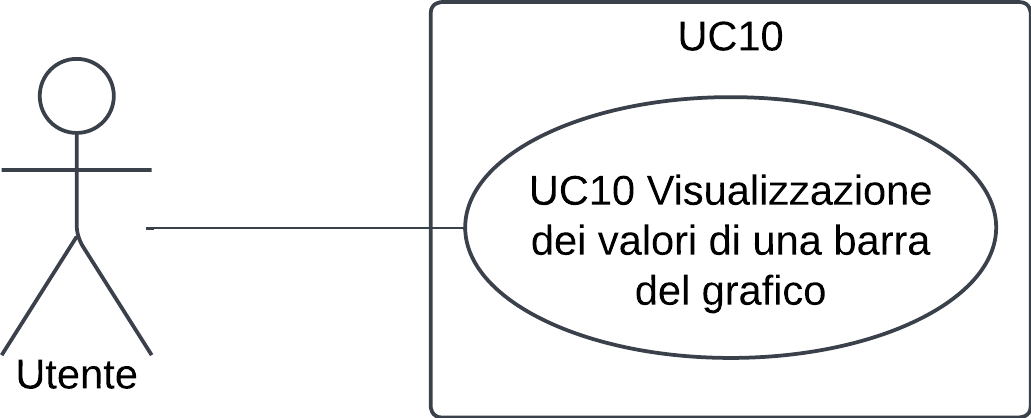
\includegraphics[scale=0.7]{template/images/UC10.png}
    \caption{\nameref*{UC:\arabic{UC}}}
\end{figure}
\UCdsc
{ % ATTORE
    \begin{itemize}
        \item Utente in ambiente 3D.
    \end{itemize}
}
{ % DESCRIZIONE
    \begin{itemize}
        \item Prevede il riposizionamento della telecamera al suo punto iniziale, la sua posizione alla creazione dell'ambiente 3D.
    \end{itemize}
}
{ % PRECONDIZIONI
    \begin{itemize}
        \item La telecamera si trova in una posizione arbitraria nello spazio.
    \end{itemize}
}
{ % POSTCONDIZIONI
    \begin{itemize}
        \item La telecamera si trova nella posizione predefinita iniziale.
    \end{itemize}
}
{ % SCENARIO PRIMARIO
    \begin{itemize}
        \item L'utente seleziona il comando per riposizionare la telecamera;
    \end{itemize}
}

\UseCase{Visualizza dettagli di una barra del grafico 3D}
\begin{figure}[h!]\centering
    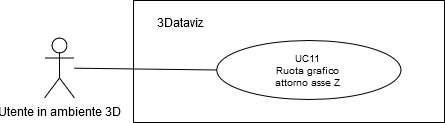
\includegraphics[scale=0.7]{template/images/UC11.png}
    \caption{\nameref*{UC:\arabic{UC}}}
\end{figure}
\UCdsc
{ % ATTORE
    \begin{itemize}
        \item Utente in ambiente 3D.
    \end{itemize}
}
{ % DESCRIZIONE
    \begin{itemize}
        \item L'utente può visualizzare i dettagli di una barra del grafico come il suo valore e le etichette a lei associate.
    \end{itemize}
}
{ % PRECONDIZIONI
    \begin{itemize}
        \item Il grafico è visibile.
        \item La barra è visibile.
    \end{itemize}
}
{ % POSTCONDIZIONI
    \begin{itemize}
        \item I dettagli della barra sono visibili.
    \end{itemize}
}
{ % SCENARIO PRIMARIO
    \begin{itemize}
        \item L'utente seleziona un valore del dataset. 
    \end{itemize}
}

\SubUseCase{Visualizza valore}
\UCdsc
{ % ATTORE
    \begin{itemize}
        \item Utente in ambiente 3D.
    \end{itemize}
}
{ % DESCRIZIONE
    \begin{itemize}
        \item Visualizzazione del valore della barra.
    \end{itemize}
}
{ % PRECONDIZIONI
    \begin{itemize}
        \item I dettagli della barra sono visibili.
    \end{itemize}
}
{ % POSTCONDIZIONI
    \begin{itemize}
        \item I dettagli della barra sono visibili.
        \item Il valore della barra è visibile.
    \end{itemize}
}
{ % SCENARIO PRIMARIO
    \begin{itemize}
        \item Nessuna azione richiesta. 
    \end{itemize}
}

\SubUseCase{Visualizza etichette}
\UCdsc
{ % ATTORE
    \begin{itemize}
        \item Utente in ambiente 3D.
    \end{itemize}
}
{ % DESCRIZIONE
    \begin{itemize}
        \item Visualizzazione delle etichette associate alla barra.
    \end{itemize}
}
{ % PRECONDIZIONI
    \begin{itemize}
        \item I dettagli della barra sono visibili.
    \end{itemize}
}
{ % POSTCONDIZIONI
    \begin{itemize}
        \item I dettagli della barra sono visibili.
        \item Le etichette della barra sono visibili.
    \end{itemize}
}
{ % SCENARIO PRIMARIO
    \begin{itemize}
        \item Nessuna azione richiesta. 
    \end{itemize}
}

\UseCase{Filtra barre}
\begin{figure}[h!]\centering
    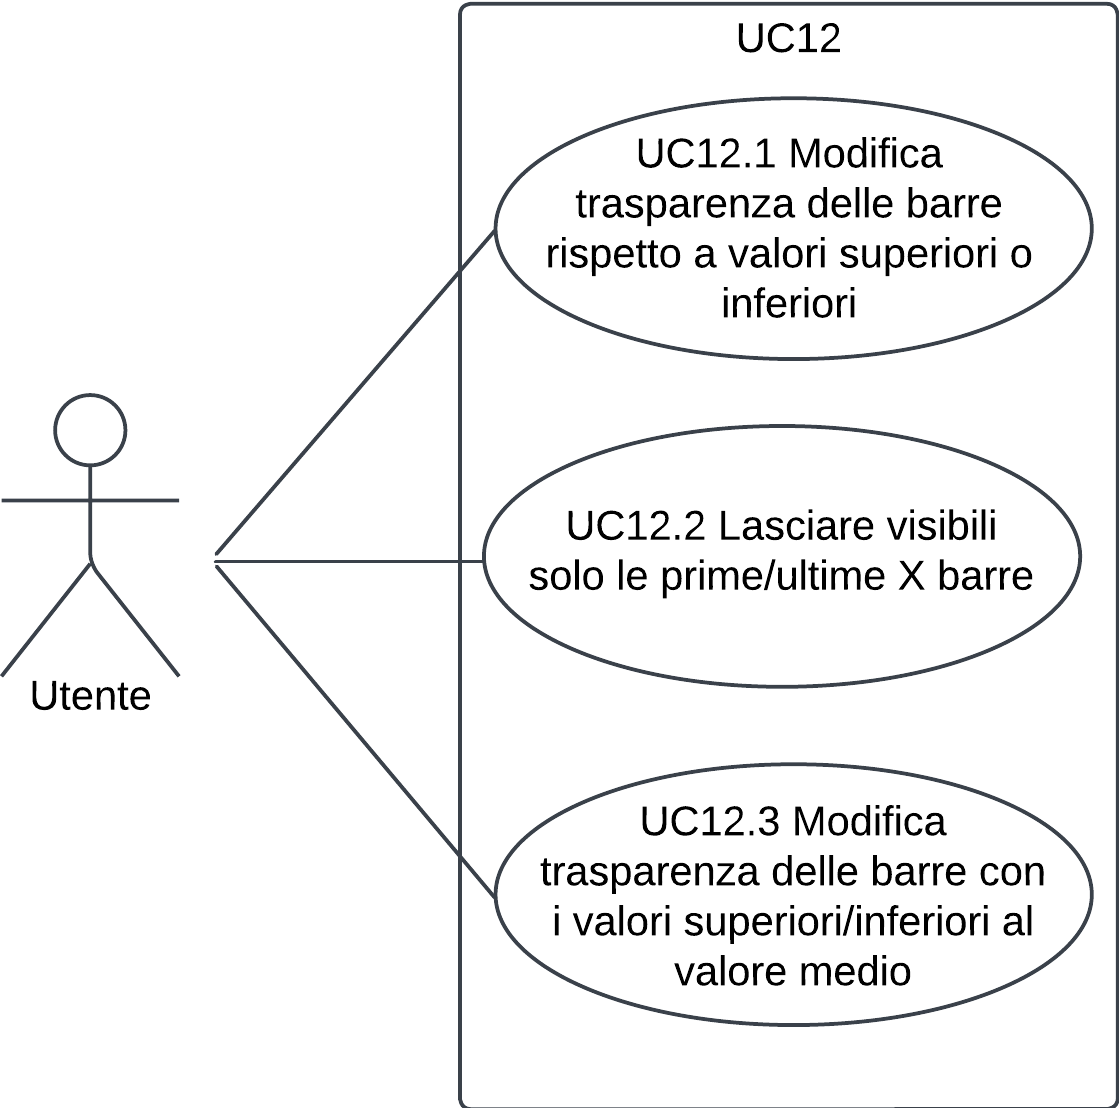
\includegraphics[scale=0.6]{template/images/UC12.png}
    \caption{\nameref*{UC:\arabic{UC}}}
\end{figure}
\UCdsc
{ % ATTORE
    \begin{itemize}
        \item Utente in ambiente 3D.
    \end{itemize}
}
{ % DESCRIZIONE
    \begin{itemize}
        \item Il filtraggio delle barre consiste nel rendere meno visibili o totalmente trasparenti le barre al di fuori del filtro selezionato dall'utente.
                Sarà l'utente a decidere quale filtro applicare.
    \end{itemize}
}
{ % PRECONDIZIONI
    \begin{itemize}
        \item Il grafico è visibile;
    \end{itemize}
}
{ % POSTCONDIZIONI
    \begin{itemize}
        \item E' stato selezionato il tipo di filtro da applicare.
    \end{itemize}
}
{ % SCENARIO PRIMARIO
    \begin{itemize}
        \item L'utente interagisce con il sistema selezionando un filtro e impostando delle regole specifiche. 
    \end{itemize}
    % GENERALIZZAZIONI
    \item \textbf{Generalizzazioni:} \begin{itemize}
        \item UC12.1 - Filtra su numero N di barre.
        \item UC12.2 - Filtra su valor medio globale.
        \item UC13 - Filtra su data barra.
    \end{itemize}
}

\SubUseCase{Filtra su numero N di barre}
\begin{figure}[h!]\centering
    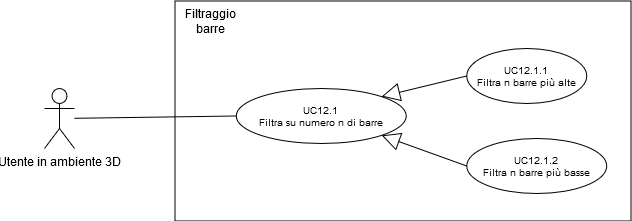
\includegraphics[scale=0.7]{template/images/UC12.1.png}
    \caption{\nameref*{UC:\arabic{UC}}}
\end{figure}
\UCdsc
{ % ATTORE
    \begin{itemize}
        \item Utente in ambiente 3D.
    \end{itemize}
}
{ % DESCRIZIONE
    \begin{itemize}
        \item Il filtraggio su numero N consiste nel tenere visibili solo le barre che rientrano tra le prime N con i valori più alti o bassi. 
                N è il numero massimo di barre da tenere in considerazione.
    \end{itemize}
}
{ % PRECONDIZIONI
    \begin{itemize}
        \item Il grafico è visibile;
    \end{itemize}
}
{ % POSTCONDIZIONI
    \begin{itemize}
        \item E' stato selezionato il filtro per tenere visibili solo le prime N barre più alte o basse.
    \end{itemize}
}
{ % SCENARIO PRIMARIO
    \begin{itemize}
        \item L'utente interagisce con il sistema selezionando il filtro per tenere visibili solo le prime N barre più alte o basse.
    \end{itemize}
        % GENERALIZZAZIONI
        \item \textbf{Generalizzazioni:} \begin{itemize}
            \item UC12.1.1 - Filtra N barre più alte.
            \item UC12.1.2 - Filtra N barre più basse.
        \end{itemize}
}

\SubSubUseCase{Filtra N barra più alte}
\UCdsc
{ % ATTORE
    \begin{itemize}
        \item Utente in ambiente 3D.
    \end{itemize}
}
{ % DESCRIZIONE
    \begin{itemize}
        \item L'utente decide di tenere visibili solo le N barre più alte.
    \end{itemize}
}
{ % PRECONDIZIONI
    \begin{itemize}
        \item Il grafico è visibile;
        \item L'utente ha scelto il filtro su numero N di barre.
    \end{itemize}
}
{ % POSTCONDIZIONI
    \begin{itemize}
        \item Le barre che non rientrano nelle prime N più alte vengono opacizzate.
    \end{itemize}
}
{ % SCENARIO PRIMARIO
    \begin{itemize}
        \item L'utente interagisce con il sistema selezionando il filtro per tenere visibili solo le prime N barre più alte.
    \end{itemize}
}

\SubSubUseCase{Filtra N barra più basse}
\UCdsc
{ % ATTORE
    \begin{itemize}
        \item Utente in ambiente 3D.
    \end{itemize}
}
{ % DESCRIZIONE
    \begin{itemize}
        \item L'utente decide di tenere visibili solo le N barre più basse.
    \end{itemize}
}
{ % PRECONDIZIONI
    \begin{itemize}
        \item Il grafico è visibile;
        \item L'utente ha scelto il filtro su numero N di barre.
    \end{itemize}
}
{ % POSTCONDIZIONI
    \begin{itemize}
        \item Le barre che non rientrano nelle prime N più basse vengono opacizzate.
    \end{itemize}
}
{ % SCENARIO PRIMARIO
    \begin{itemize}
        \item L'utente interagisce con il sistema selezionando il filtro per tenere visibili solo le prime N barre più basse.
    \end{itemize}
}


\SubUseCase{Filtra su valor medio globale}
\begin{figure}[h!]\centering
    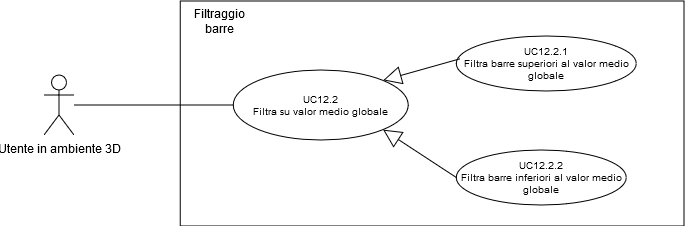
\includegraphics[scale=0.65]{template/images/UC12.2.png}
    \caption{\nameref*{UC:\arabic{UC}}}
\end{figure}
\UCdsc
{ % ATTORE
    \begin{itemize}
        \item Utente in ambiente 3D.
    \end{itemize}
}
{ % DESCRIZIONE
    \begin{itemize}
        \item Il filtraggio su valor medio globale consiste nel tenere visibili le barre più alte o più basse rispetto al valor medio globale.
    \end{itemize}
}
{ % PRECONDIZIONI
    \begin{itemize}
        \item Il grafico è visibile;
    \end{itemize}
}
{ % POSTCONDIZIONI
    \begin{itemize}
        \item E' stato selezionato il filtro sul valor medio.
    \end{itemize}
}
{ % SCENARIO PRIMARIO
    \begin{itemize}
        \item L'utente interagisce con il sistema selezionando il filtro per tenere visibili solo le barre più alte o più basse rispetto al valor medio globale.
    \end{itemize}
        % GENERALIZZAZIONI
        \item \textbf{Generalizzazioni:} \begin{itemize}
            \item UC12.2.1 - Filtra barre superiori al valor medio globale.
            \item UC12.2.2 - Filtra barre inferiori al valor medio globale.
        \end{itemize}
}

\SubSubUseCase{Filtra barre superiori al valor medio globale}
\UCdsc
{ % ATTORE
    \begin{itemize}
        \item Utente in ambiente 3D.
    \end{itemize}
}
{ % DESCRIZIONE
    \begin{itemize}
        \item L'utente decide di tenere visibili barre con un valore superiore al valor medio globale.
    \end{itemize}
}
{ % PRECONDIZIONI
    \begin{itemize}
        \item Il grafico è visibile;
        \item L'utente ha scelto il filtro su valor medio.
    \end{itemize}
}
{ % POSTCONDIZIONI
    \begin{itemize}
        \item Le barre inferiori al valor medio globale vengono opacizzate.
    \end{itemize}
}
{ % SCENARIO PRIMARIO
    \begin{itemize}
        \item L'utente interagisce con il sistema selezionando il filtro per tenere visibili le barre che hanno un valore superiore al valor medio globale.
    \end{itemize}
}

\SubSubUseCase{Filtra barre inferiori al valor medio globale}
\UCdsc
{ % ATTORE
    \begin{itemize}
        \item Utente in ambiente 3D.
    \end{itemize}
}
{ % DESCRIZIONE
    \begin{itemize}
        \item L'utente decide di tenere visibili barre con un valore inferiore al valor medio globale.
    \end{itemize}
}
{ % PRECONDIZIONI
    \begin{itemize}
        \item Il grafico è visibile;
        \item L'utente ha scelto il filtro su valor medio.
    \end{itemize}
}
{ % POSTCONDIZIONI
    \begin{itemize}
        \item Le barre superiori al valor medio globale vengono opacizzate.
    \end{itemize}
}
{ % SCENARIO PRIMARIO
    \begin{itemize}
        \item L'utente interagisce con il sistema selezionando il filtro per tenere visibili le barre che hanno un valore inferiore al valor medio globale.
    \end{itemize}
}


\UseCase{Filtra su una data barra}
\begin{figure}[h!]\centering
    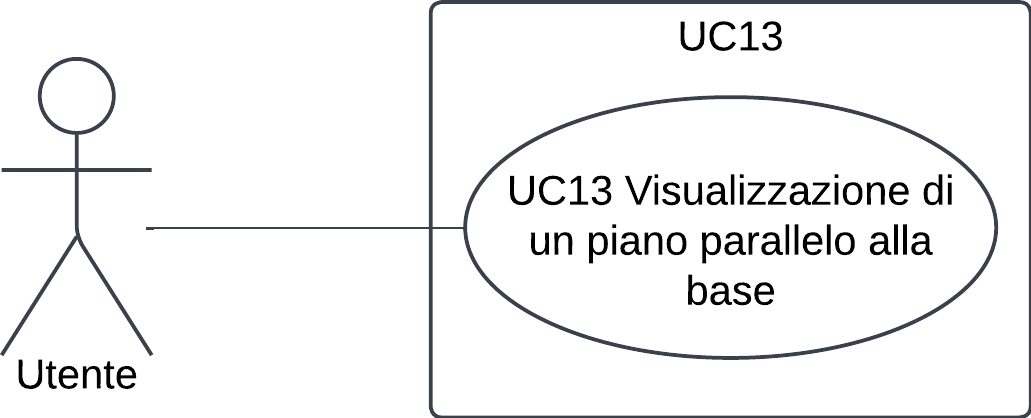
\includegraphics[scale=0.7]{template/images/UC13.png}
    \caption{\nameref*{UC:\arabic{UC}}}
\end{figure}
\UCdsc
{ % ATTORE
    \begin{itemize}
        \item Utente in ambiente 3D.
    \end{itemize}
}
{ % DESCRIZIONE
    \begin{itemize}
        \item Il filtraggio su una data barra consiste nel tenere visibili solo le altre barre che hanno un valore superiore o inferiore rispetto ad una barra scelta dall'utente.
    \end{itemize}
}
{ % PRECONDIZIONI
    \begin{itemize}
        \item Il grafico è visibile;
    \end{itemize}
}
{ % POSTCONDIZIONI
    \begin{itemize}
        \item E' stato selezionato il filtro per tenere visibili solo le barre con un valore superiore o inferiore rispetto ad una barra scelta dall'utente.
    \end{itemize}
}
{ % SCENARIO PRIMARIO
    \begin{itemize}
        \item L'utente seleziona un valore del dataset che corrisponde ad una barra sul grafico 3D.
    \end{itemize}
     % GENERALIZZAZIONI
     \item \textbf{Generalizzazioni:} \begin{itemize}
        \item UC13.1 - Filtra barre superiori a una data barra.
        \item UC13.2 - Filtra barre inferiori a una data barra.
    \end{itemize}
}

\SubUseCase{Filtra barre superiori a una data barra}
\UCdsc
{ % ATTORE
    \begin{itemize}
        \item Utente in ambiente 3D.
    \end{itemize}
}
{ % DESCRIZIONE
    \begin{itemize}
        \item L'utente decide di tenere visibili solo le barre con valori superiori ad una determinata barra.
    \end{itemize}
}
{ % PRECONDIZIONI
    \begin{itemize}
        \item Il grafico è visibile;
        \item L'utente ha scelto il filtro su una data barra;
    \end{itemize}
}
{ % POSTCONDIZIONI
    \begin{itemize}
        \item Le barre inferiori rispetto al valore di una determinata barra vengono opacizzate.
    \end{itemize}
}
{ % SCENARIO PRIMARIO
    \begin{itemize}
        \item L'utente interagisce con il sistema selezionando il filtro per tenere visibili le barre che hanno un valore superiore rispetto al valore di una determinata barra.
    \end{itemize}
}

\SubUseCase{Filtra barre inferiori a una data barra}
\UCdsc
{ % ATTORE
    \begin{itemize}
        \item Utente in ambiente 3D.
    \end{itemize}
}
{ % DESCRIZIONE
    \begin{itemize}
        \item L'utente decide di tenere visibili solo le barre con valori inferiori ad una determinata barra.
    \end{itemize}
}
{ % PRECONDIZIONI
    \begin{itemize}
        \item Il grafico è visibile;
        \item L'utente ha scelto il filtro su una data barra;
    \end{itemize}
}
{ % POSTCONDIZIONI
    \begin{itemize}
        \item Le barre superiori rispetto al valore di una determinata barra vengono opacizzate.
    \end{itemize}
}
{ % SCENARIO PRIMARIO
    \begin{itemize}
        \item L'utente interagisce con il sistema selezionando il filtro per tenere visibili le barre che hanno un valore inferiori rispetto al valore di una determinata barra.
    \end{itemize}
}

\UseCase{Visualizza barra in primo piano}
\begin{figure}[h!]\centering
    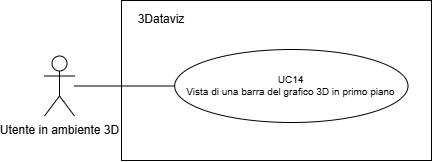
\includegraphics[scale=0.7]{template/images/UC14.png}
    \caption{\nameref*{UC:\arabic{UC}}}
\end{figure}
\UCdsc
{ % ATTORE
    \begin{itemize}
        \item Utente in ambiente 3D.
    \end{itemize}
}
{ % DESCRIZIONE
    \begin{itemize}
        \item La visualizzazione di una barra in primo piano consiste nel posizionare la telecamera in modo da massimizzare la visibilità di una specifica barra all'interno della scena, garantendo che sia sempre presente nel campo visivo dell'utente.
    \end{itemize}
}
{ % PRECONDIZIONI
    \begin{itemize}
        \item Il grafico è visibile;
        \item La telecamera è in una posizione arbitraria;
        \item \item L'utente seleziona un valore del dataset.
    \end{itemize}
}
{ % POSTCONDIZIONI
    \begin{itemize}
        \item La telecamera si trova in una posizione diversa da quella di partenza.
    \end{itemize}
}
{ % SCENARIO PRIMARIO
    \begin{itemize}
        \item L'utente seleziona un valore del dataset che corrisponde ad una barra sul grafico 3D.
    \end{itemize}
}


\UseCase{Ripristina stato del grafico}
\begin{figure}[h!]\centering
    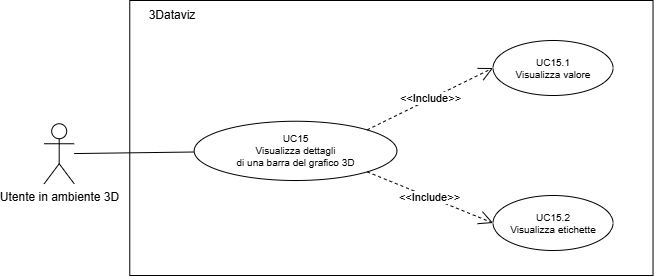
\includegraphics[scale=0.7]{template/images/UC15.png}
    \caption{\nameref*{UC:\arabic{UC}}}
\end{figure}
\UCdsc
{ % ATTORE
    \begin{itemize}
        \item Utente in ambiente 3D.
    \end{itemize}
    }
    { % DESCRIZIONE
    \begin{itemize}
        \item Consiste nel togliere il filtro applicato al grafico e far tornare le barre al loro stile originale.
    \end{itemize}
}
{ % PRECONDIZIONI
    \begin{itemize}
        \item Il grafico è visibile;
    \end{itemize}
}
{ % POSTCONDIZIONI
    \begin{itemize}
        \item I filtri vengono rimossi;
        \item Le barre del grafico tornano allo stile originale.
    \end{itemize}
}
{ % SCENARIO PRIMARIO
    \begin{itemize}
        \item L'utente seleziona l'opzione di ripristino stato del grafico.
    \end{itemize}
}



\UseCase{Visualizza piano valor medio globale}
\begin{figure}[h!]\centering
    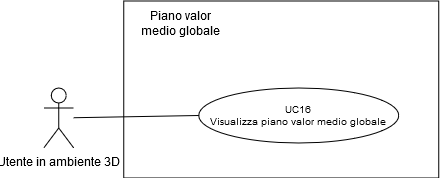
\includegraphics[scale=0.7]{template/images/UC16.png}
    \caption{\nameref*{UC:\arabic{UC}}}
\end{figure}
\UCdsc
{ % ATTORE
    \begin{itemize}
        \item Utente in ambiente 3D.
    \end{itemize}
}
{ % DESCRIZIONE
    \begin{itemize}
        \item Un piano, parallelo alla base, viene inserito nel grafico 3D per evidenziare il valor medio globale.
    \end{itemize}
}
{ % PRECONDIZIONI
    \begin{itemize}
        \item Il grafico è visibile;
    \end{itemize}
}
{ % POSTCONDIZIONI
    \begin{itemize}
        \item Il piano che rappresenta il valor medio globale è visibile.
    \end{itemize}
}
{ % SCENARIO PRIMARIO
    \begin{itemize}
        \item L'utente seleziona l'opzione per visualizzare il valor medio.
    \end{itemize}
}

\UseCase{Visualizza piano valor medio di un singolo elemento}
\begin{figure}[h!]\centering
    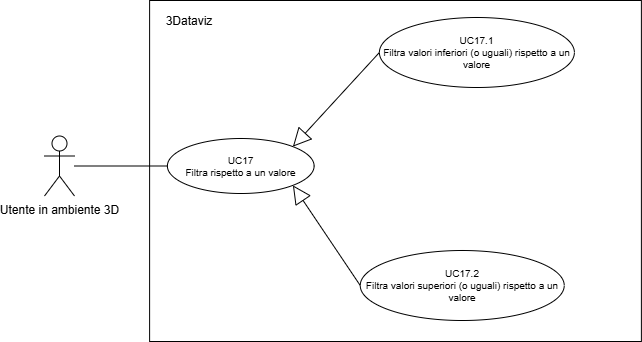
\includegraphics[scale=0.7]{template/images/UC17.png}
    \caption{\nameref*{UC:\arabic{UC}}}
\end{figure}
\UCdsc
{ % ATTORE
    \begin{itemize}
        \item Utente in ambiente 3D.
    \end{itemize}
}
{ % DESCRIZIONE
    \begin{itemize}
        \item Un piano, parallelo alla base, viene inserito nel grafico 3D per evidenziare il valor medio di un singolo elemento tra quelli nel dataset.
    \end{itemize}
}
{ % PRECONDIZIONI
    \begin{itemize}
        \item Il grafico è visibile;
    \end{itemize}
}
{ % POSTCONDIZIONI
    \begin{itemize}
        \item Il piano che rappresenta il valor medio di un singolo elemento è visibile.
    \end{itemize}
}
{ % SCENARIO PRIMARIO
    \begin{itemize}
        \item L'utente seleziona l'opzione per visualizzare il valor medio.
        \item L'utente seleziona l'elemento su quale andare a calcolare il valor medio.
    \end{itemize}
}

